\likeechapter{Приложение А}
\appendix
\counterwithout{figure}{chapter}
\setcounter{figure}{0}
\begin{figure}[H]
	\centering
	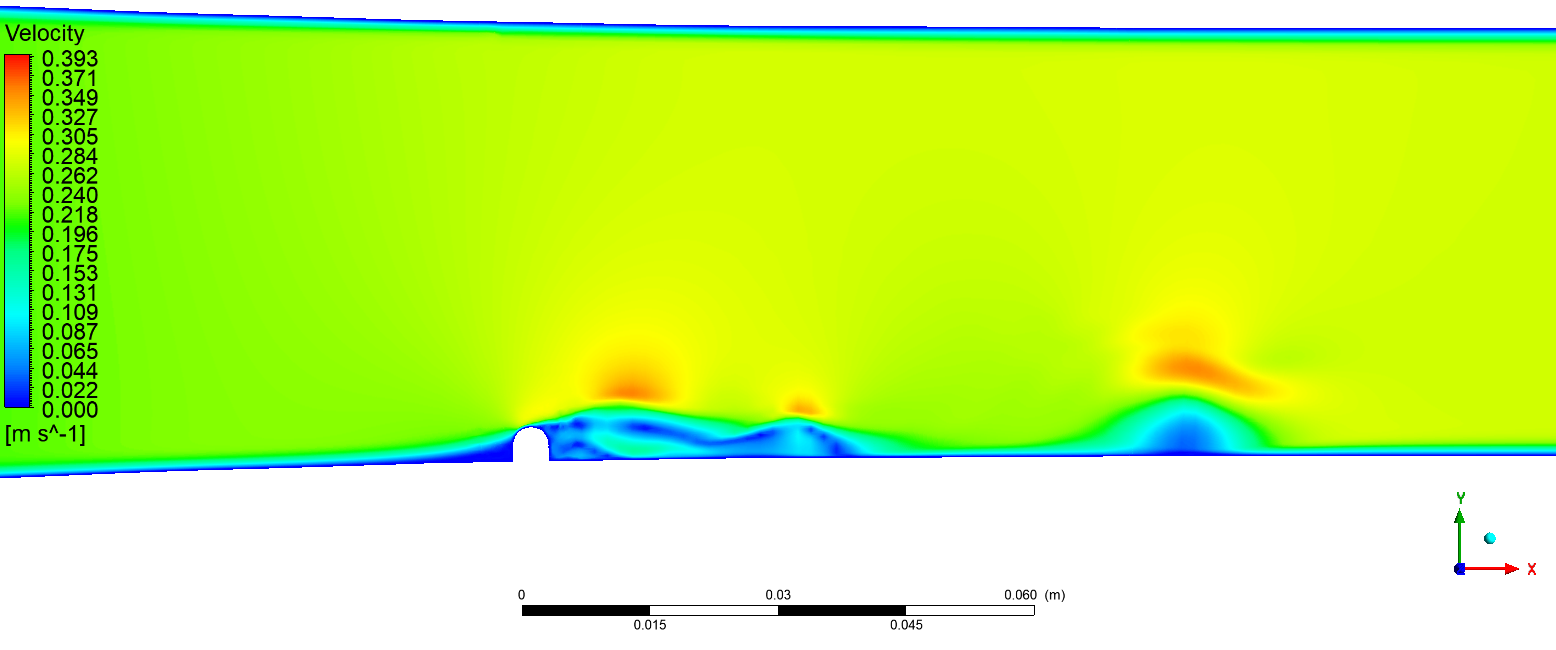
\includegraphics[width=0.9\linewidth]{../Assets/T0_Velocity_ContourXY}
	\caption{PlaneXY, t = 0.6 c}
	\label{fig:t0velocitycontourxy}
\end{figure}
\begin{figure}[H]
	\begin{subfigure}{.5\textwidth}
		\centering
		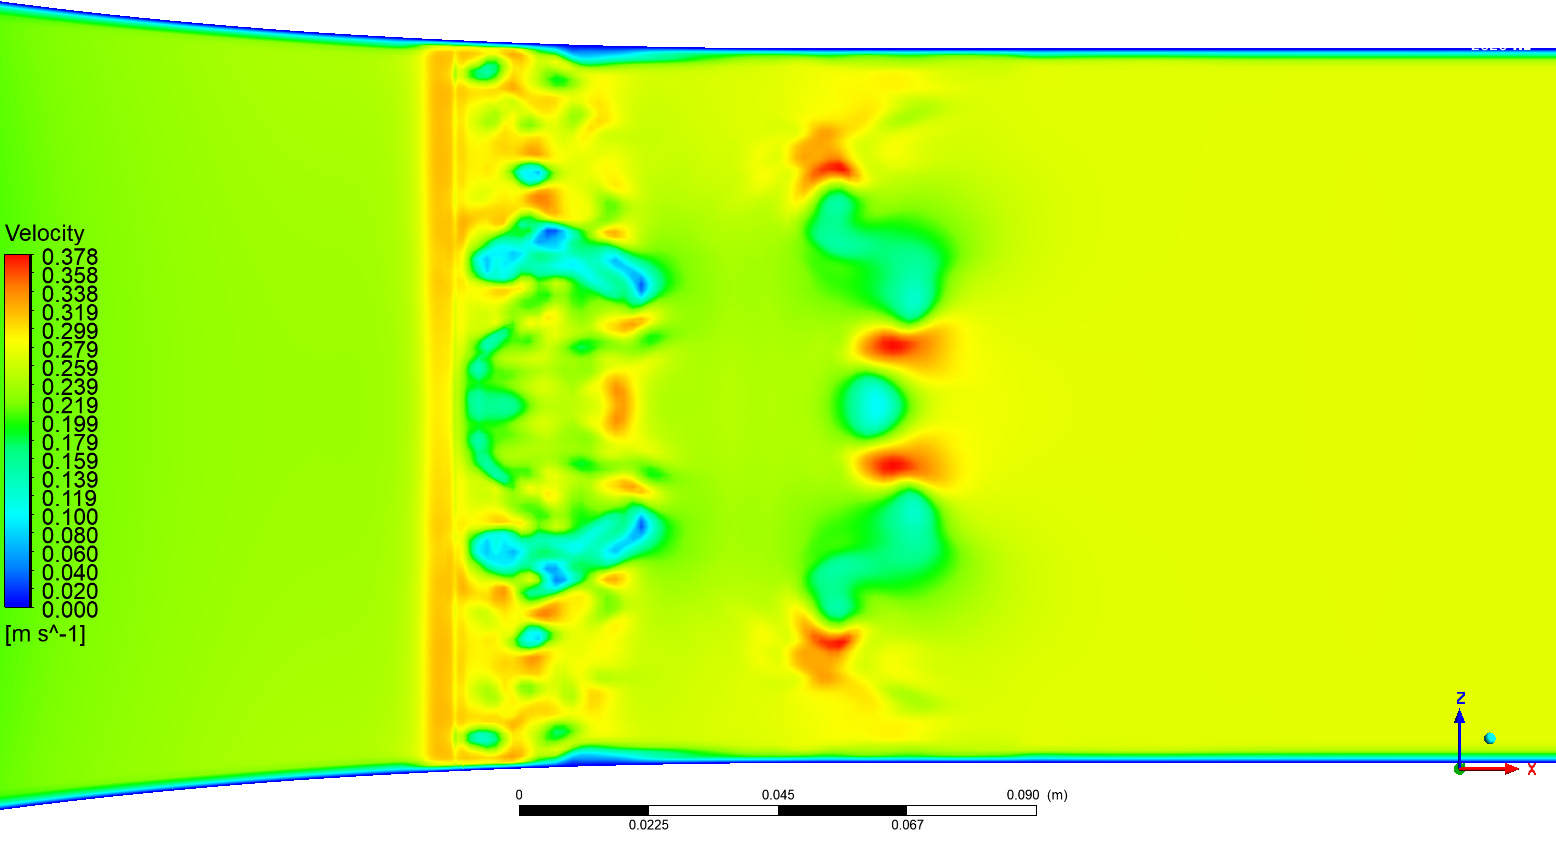
\includegraphics[width=1.7\linewidth, angle=90]{../Assets/T0_Velocity_ContourXZ20M}
		\caption{PlaneXZ20M}
		\label{fig:t0velocitycontourxz20m}
	\end{subfigure}%
	\begin{subfigure}{.5\textwidth}
		\centering
		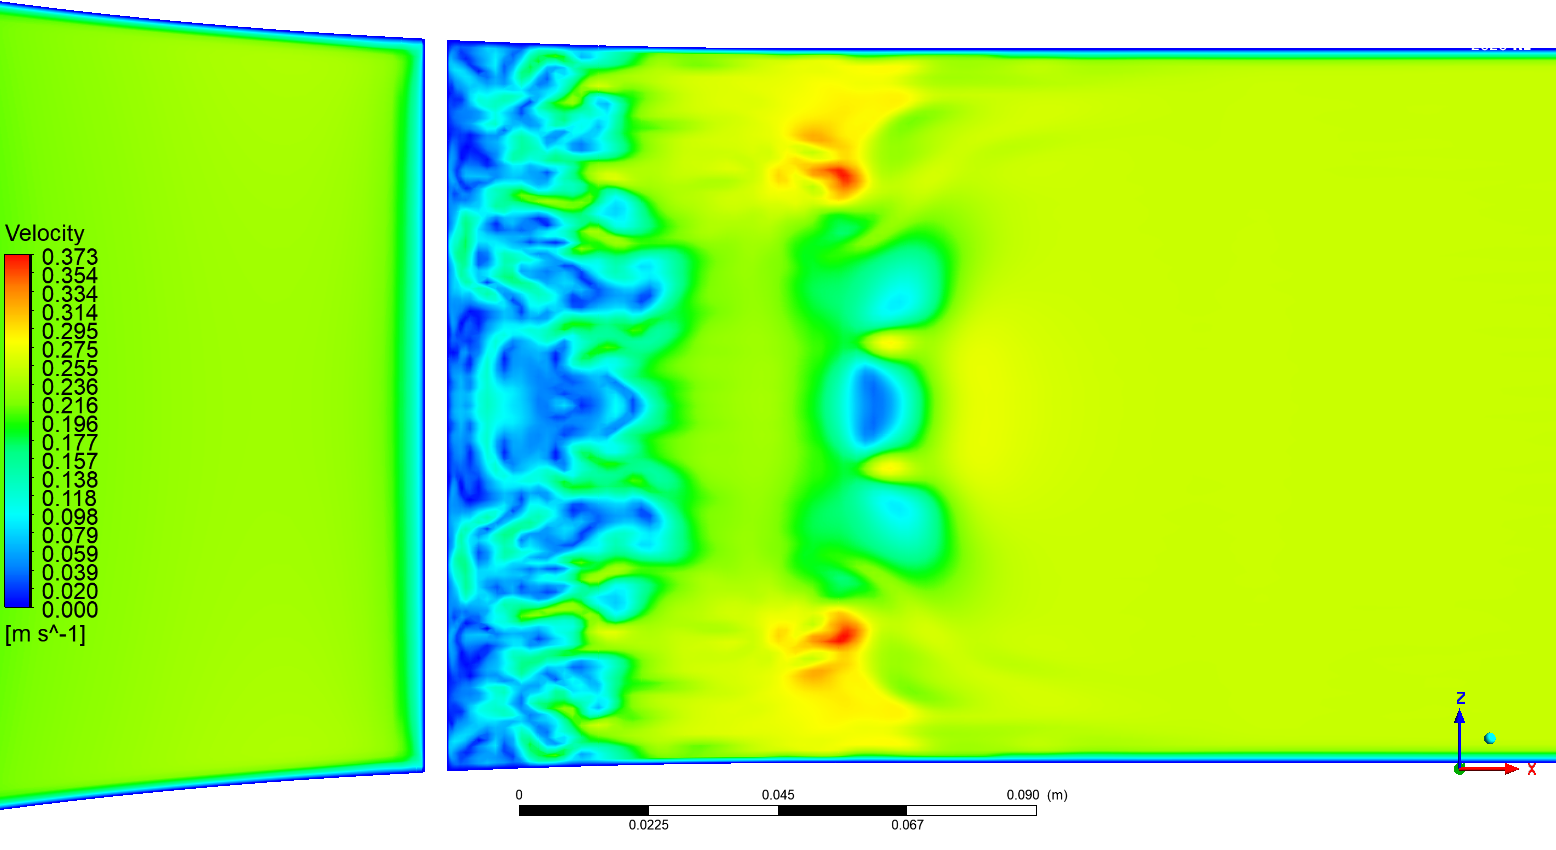
\includegraphics[width=1.7\linewidth, angle=90]{../Assets/T0_Velocity_ContourXZ23M}
		\caption{PlaneXZ23M}
		\label{fig:t0velocitycontourxz23m}
	\end{subfigure}
		\caption{PlaneXZ, t = 0.6 c}
		\label{fig:t0velocitycontourxz}
\end{figure}
\newpage
\begin{flushright}
	\MakeUppercase{\textbf{Приложение А}}
\end{flushright}
\begin{figure}[H]
	\centering
	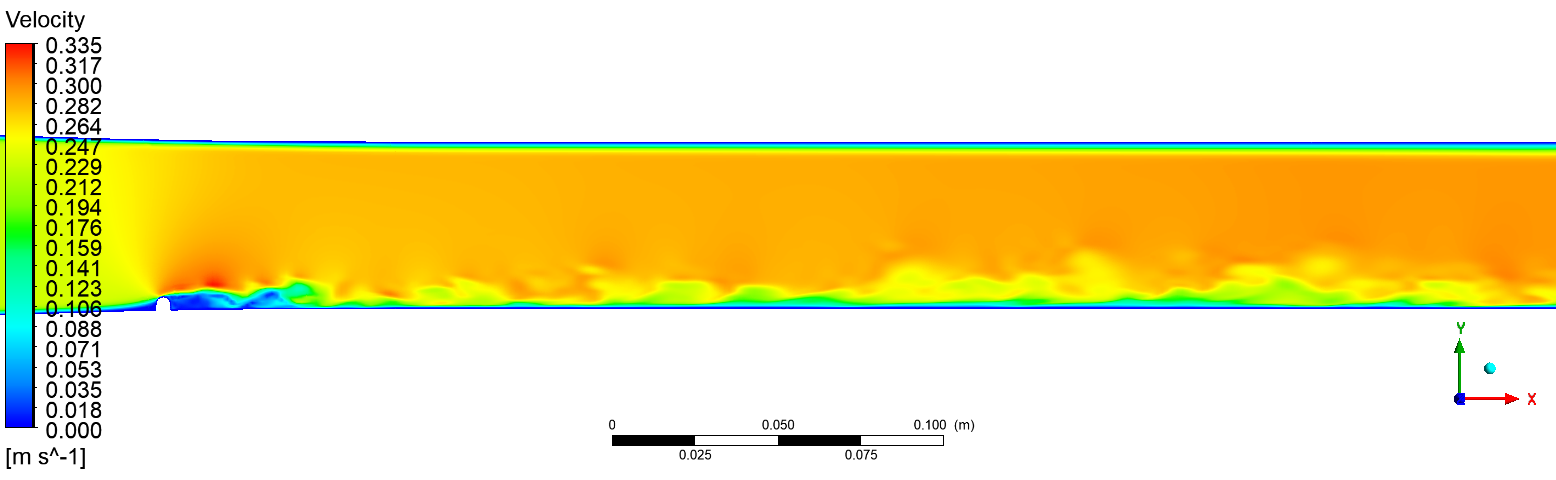
\includegraphics[width=0.9\linewidth]{../Assets/T1060_Velocity_ContourXY}
	\caption{PlaneXY, t = 10.6 c}
	\label{fig:t1060velocitycontourxy}
\end{figure}
\begin{figure}[H]
	\begin{subfigure}{.5\textwidth}
		\centering
		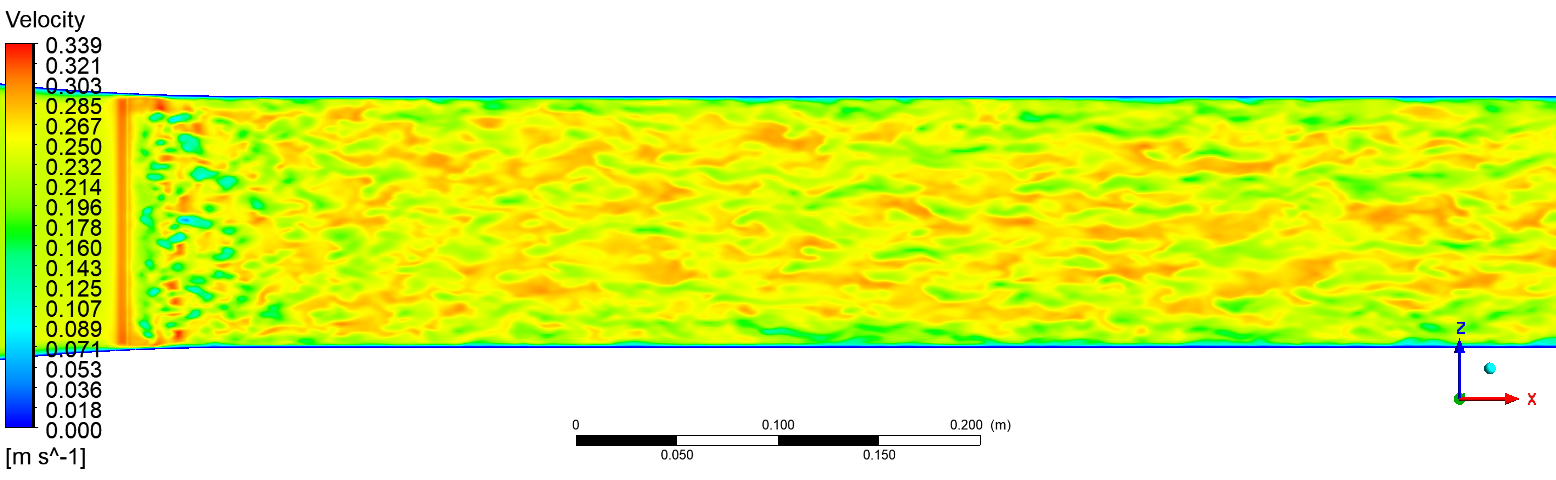
\includegraphics[width=1.7\linewidth, angle=90]{../Assets/T1060_Velocity_ContourXZ20M}
		\caption{PlaneXZ20M}
		\label{fig:t1060velocitycontourxz20m}
	\end{subfigure}%
	\begin{subfigure}{.5\textwidth}
		\centering
		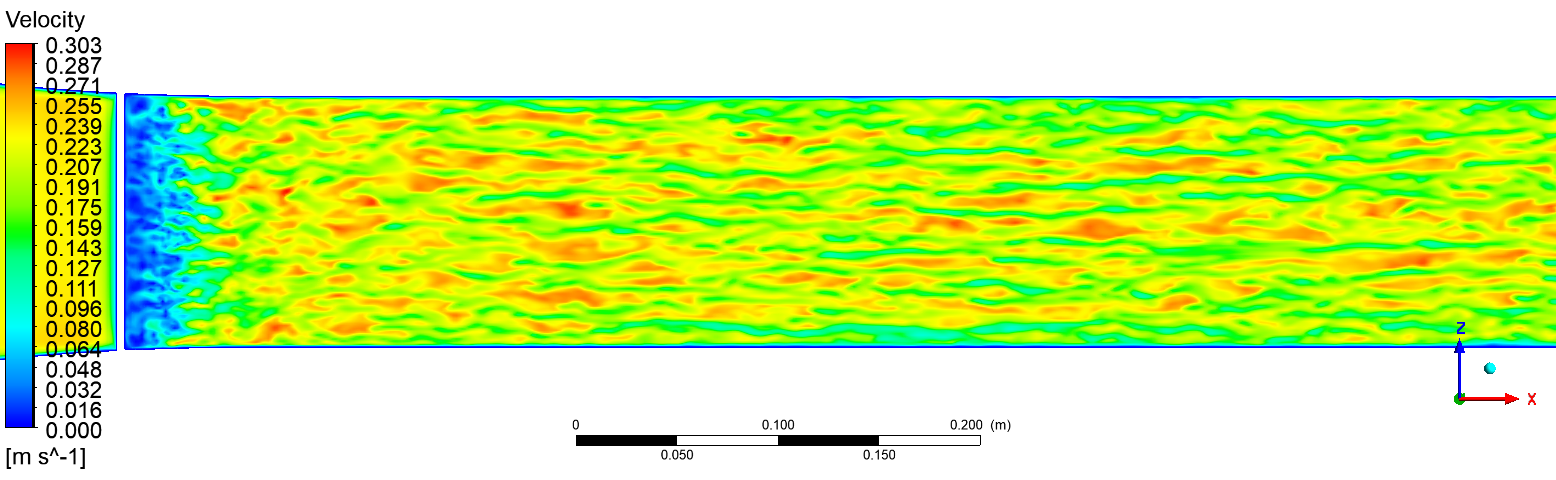
\includegraphics[width=1.7\linewidth, angle=90]{../Assets/T1060_Velocity_ContourXZ23M}
		\caption{PlaneXZ23M}
		\label{fig:t1060velocitycontourxz23m}
	\end{subfigure}
	\caption{PlaneXZ, t = 10.6 c}
	\label{fig:t1060velocitycontourxz}
\end{figure}
\newpage
\begin{flushright}
	\MakeUppercase{\textbf{Приложение А}}
\end{flushright}
\begin{figure}[H]
	\centering
	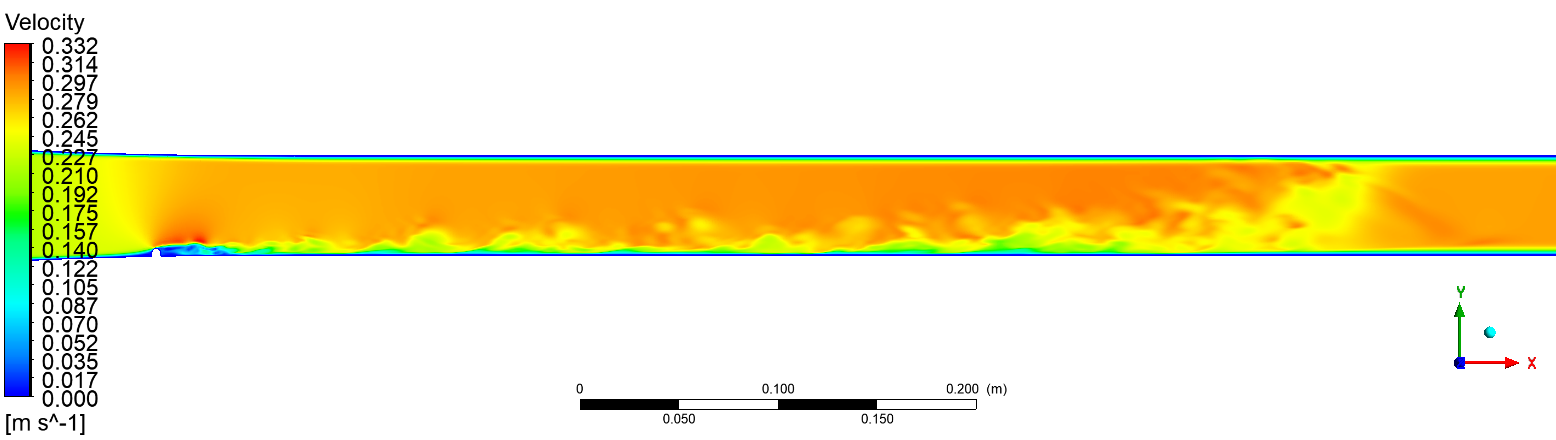
\includegraphics[width=1\linewidth]{../Assets/T265_Velocity_ContourXY}
	\caption{PlaneXY, t = 2.65 с}
	\label{fig:t265velocitycontourxy}
\end{figure}
\begin{figure}[H]
	\begin{subfigure}{.5\textwidth}
		\centering
		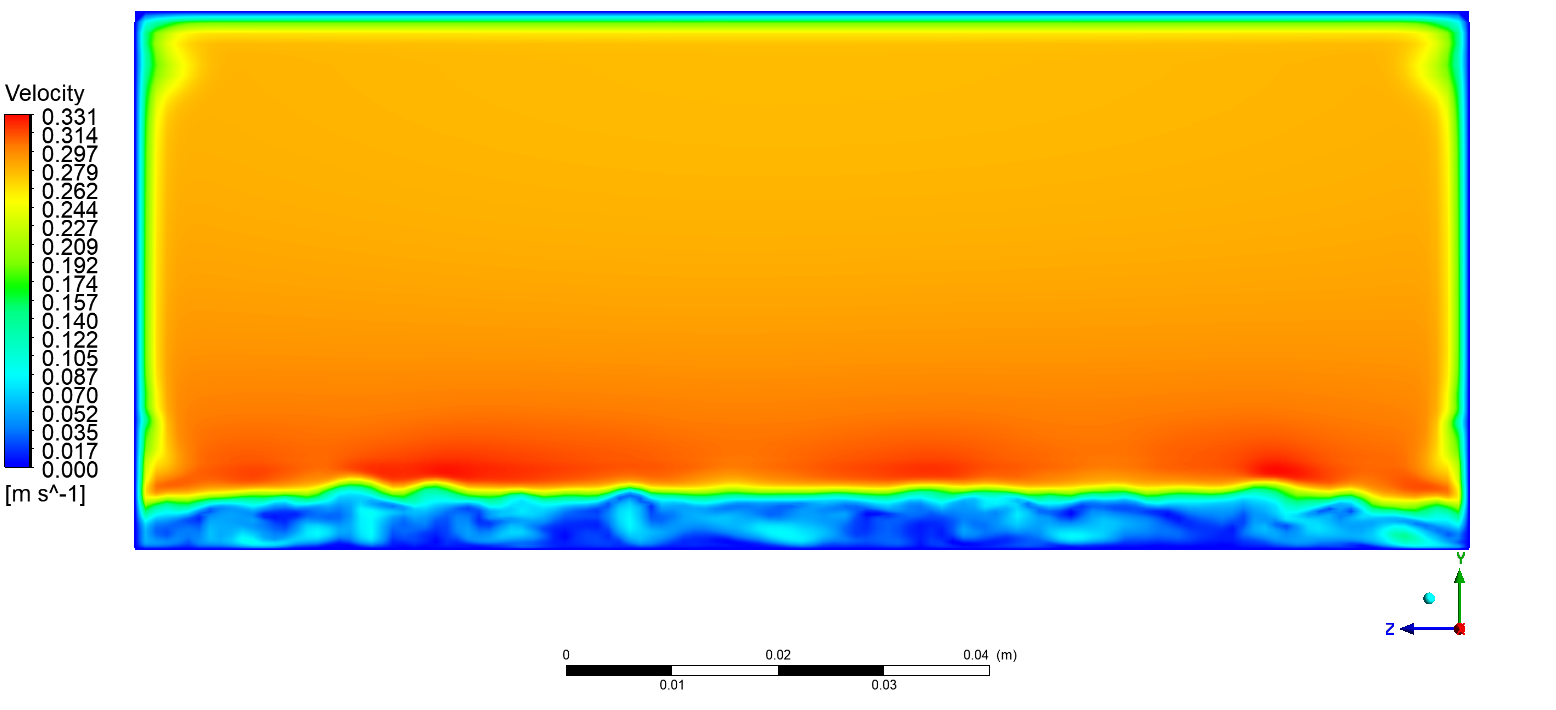
\includegraphics[width=1.1\linewidth]{../Assets/T265_Velocity_ContourYZ340}
		\caption{PlaneYZ340}
		\label{fig:T265VelocityContourYZ340}
	\end{subfigure}%
	\begin{subfigure}{.5\textwidth}
		\centering
		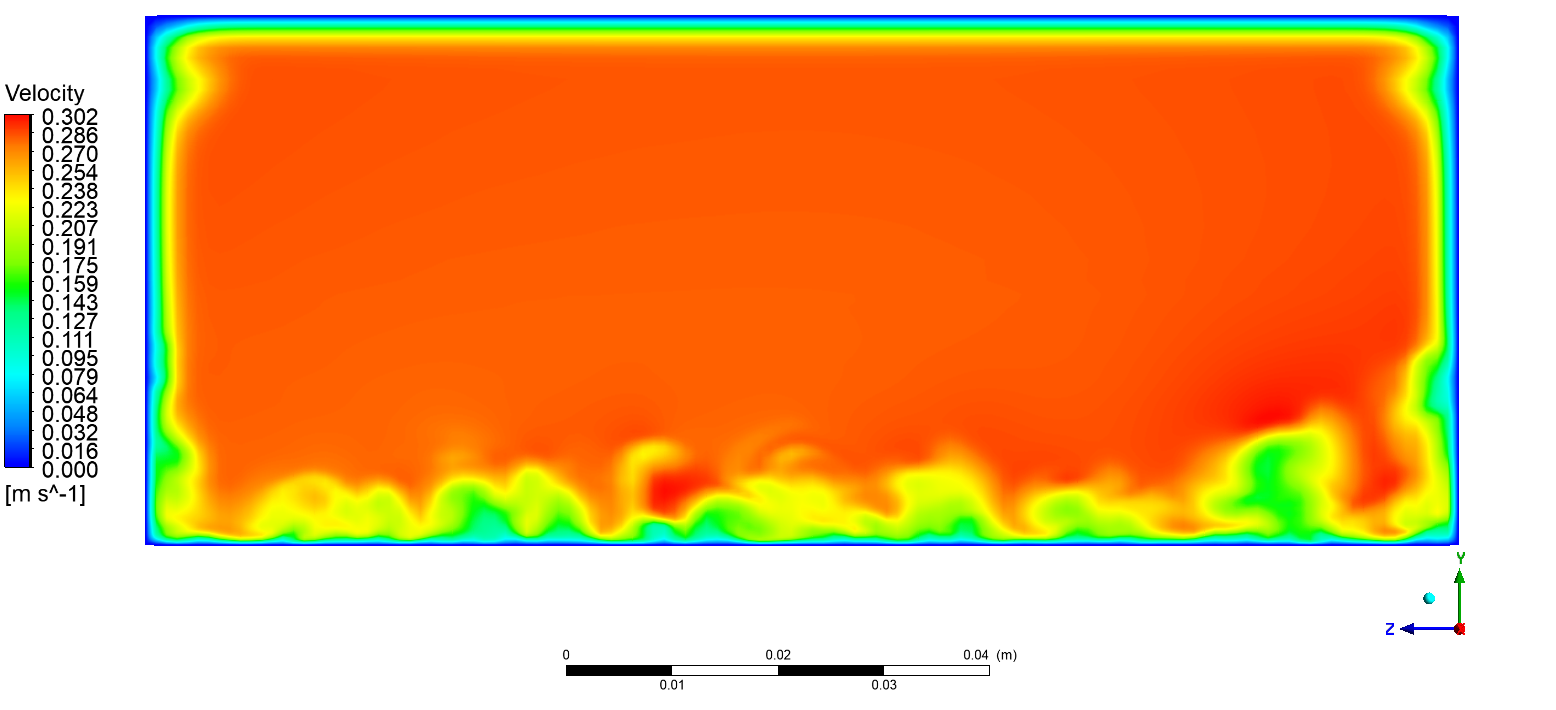
\includegraphics[width=1.1\linewidth]{../Assets/T265_Velocity_ContourYZ400}
		\caption{PlaneYZ400}
		\label{fig:T265VelocityContourYZ400}
	\end{subfigure}
	\\
	\begin{subfigure}{.5\textwidth}
		\centering
		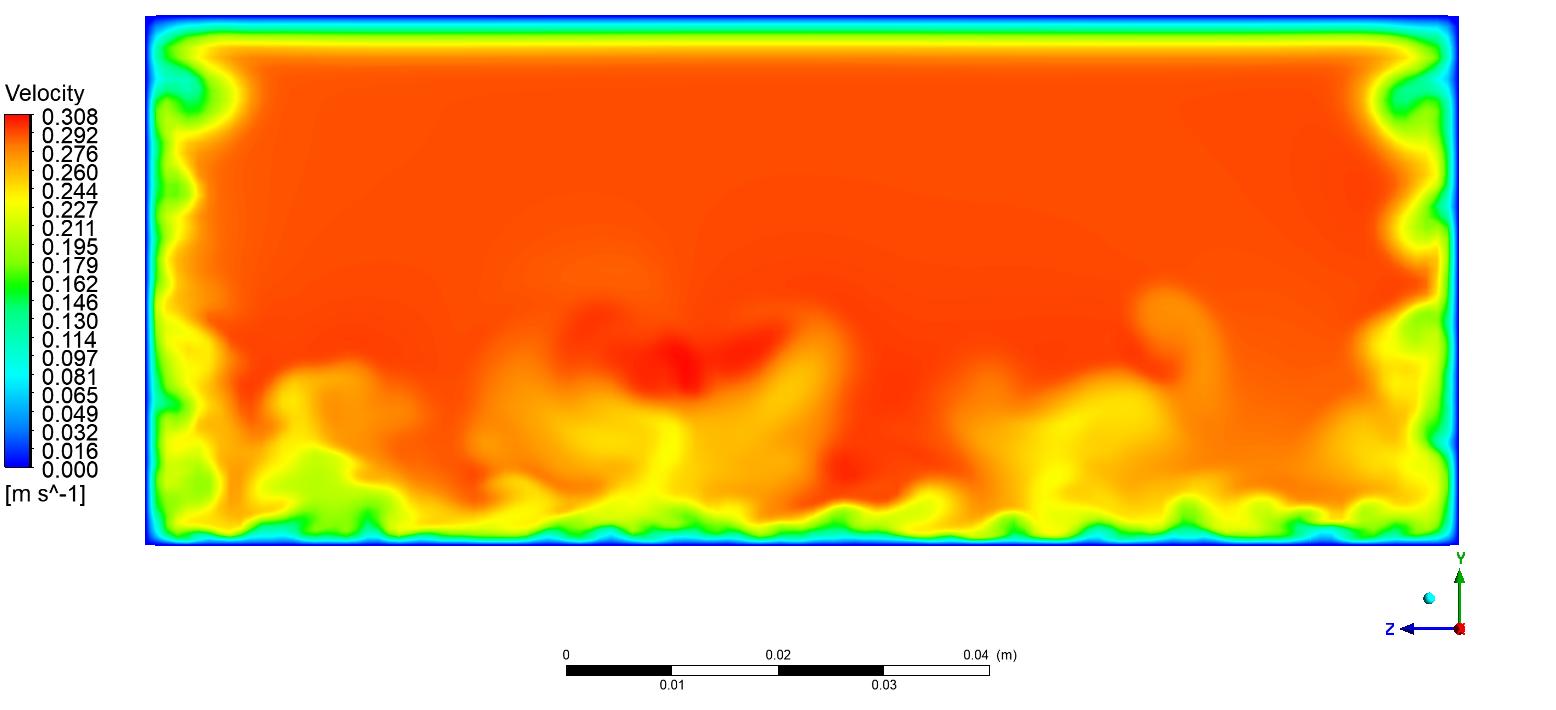
\includegraphics[width=1.1\linewidth]{../Assets/T265_Velocity_ContourYZ600}
		\caption{PlaneYZ600}
		\label{fig:T265VelocityContourYZ600}
	\end{subfigure}%
	\begin{subfigure}{.5\textwidth}
		\centering
		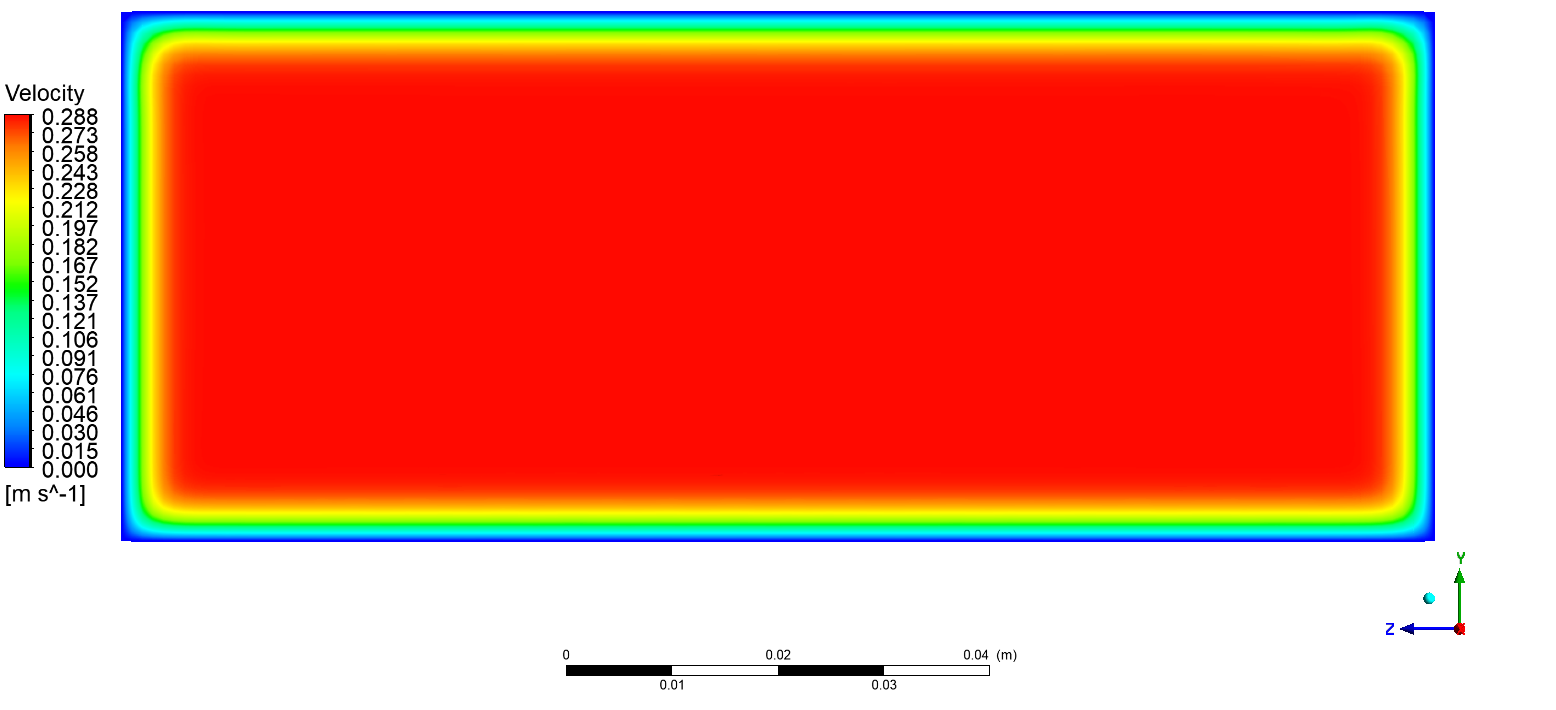
\includegraphics[width=1.1\linewidth]{../Assets/T265_Velocity_ContourYZ1400}
		\caption{PlaneYZ1400}
		\label{fig:T265VelocityContourYZ1400}
	\end{subfigure}
	\caption{Скорость в поперечных сечениях при t = 2.65 с}
	\label{fig:T265VelocityContourYZ}
\end{figure}
\begin{figure}[H]
	\centering
	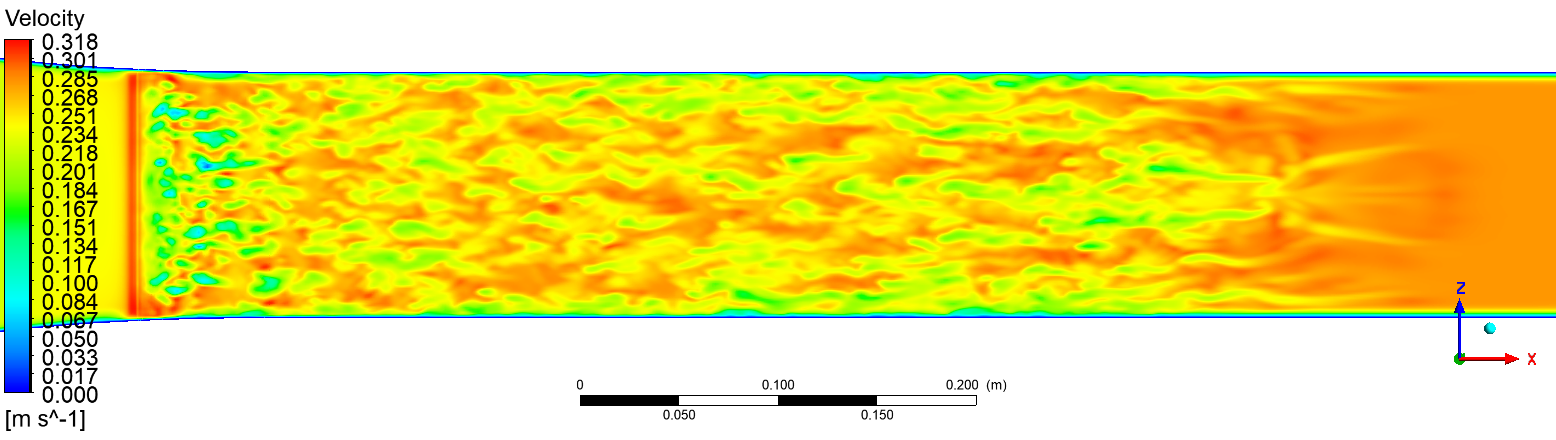
\includegraphics[width=1\linewidth]{../Assets/T265_Velocity_ContourXZ20M}
	\caption{PlaneXZ20M, t = 2.65 с}
	\label{fig:t265velocitycontourxz20m}
\end{figure}
\newpage
\begin{flushright}
	\MakeUppercase{\textbf{Приложение А}}
\end{flushright}
\begin{figure}[H]
	\centering
	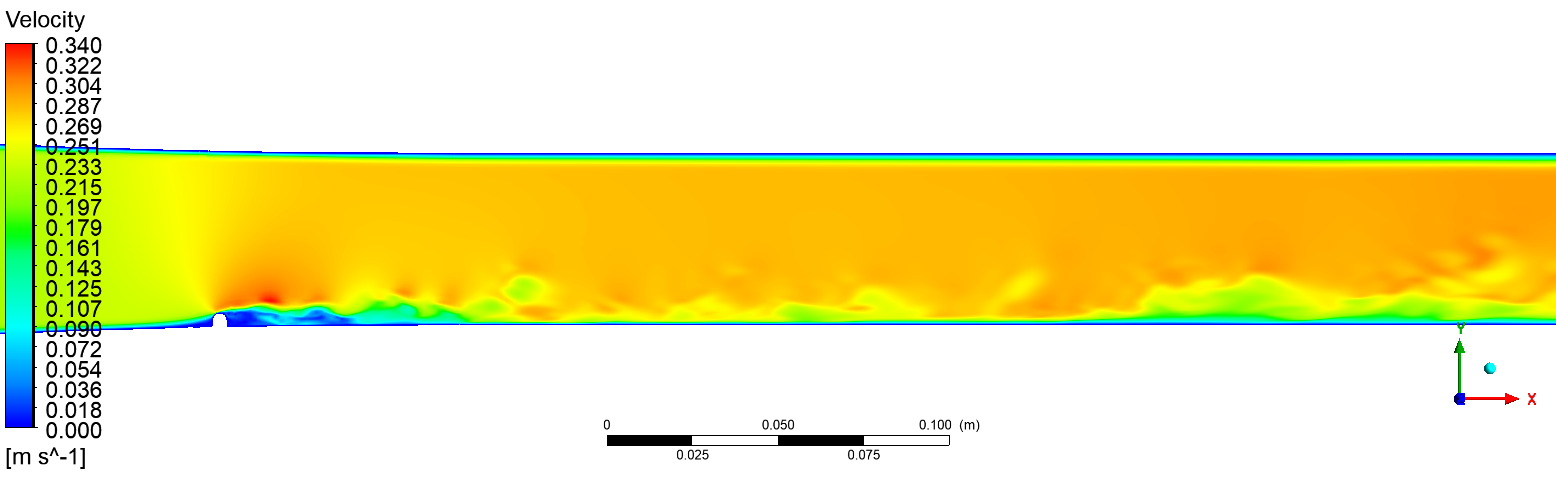
\includegraphics[width=1\linewidth]{../Assets/T665_Velocity_ContourXY}
	\caption{PlaneXY, t = 6.65 с}
	\label{fig:t665velocitycontourxy}
\end{figure}
\begin{figure}[H]
	\begin{subfigure}{.5\textwidth}
		\centering
		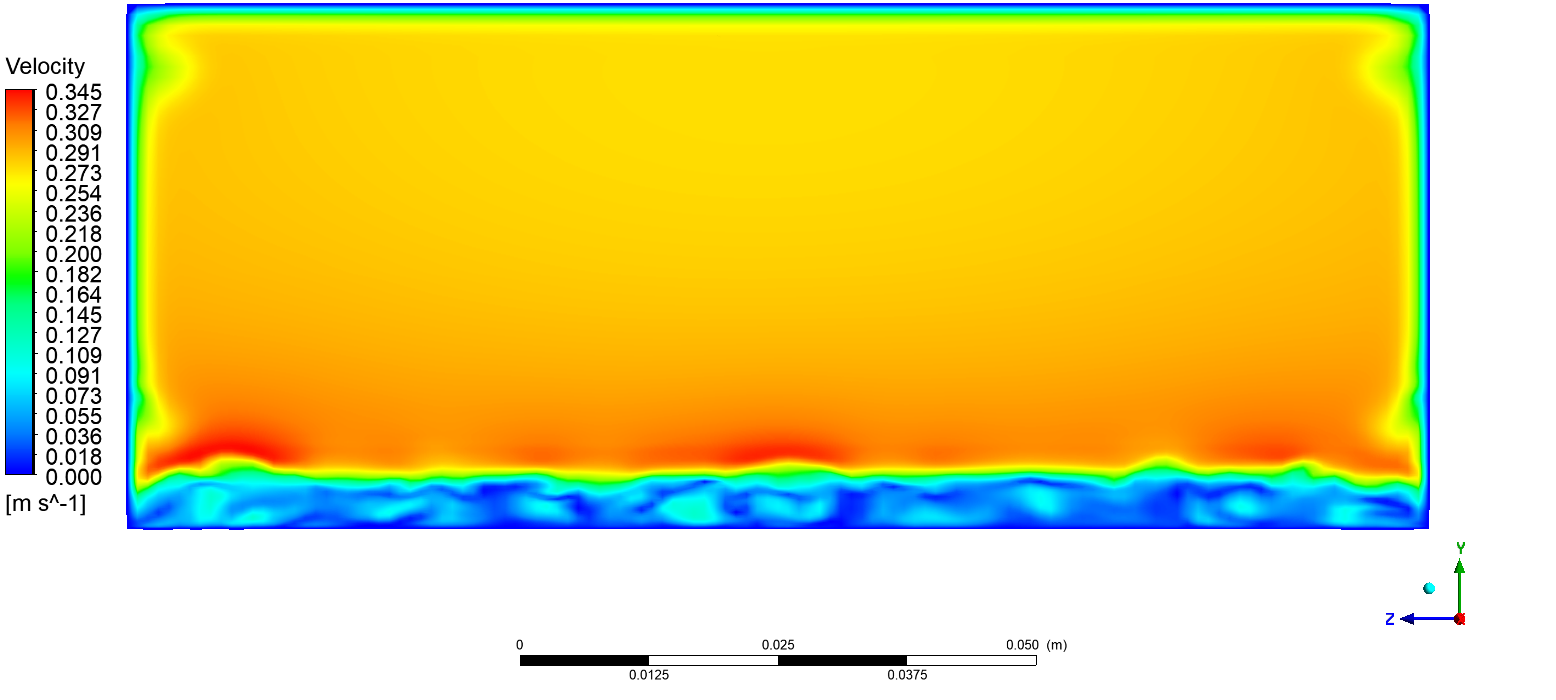
\includegraphics[width=1.1\linewidth]{../Assets/T665_Velocity_ContourYZ340}
		\caption{PlaneYZ340}
		\label{fig:T665VelocityContourYZ340}
	\end{subfigure}%
	\begin{subfigure}{.5\textwidth}
		\centering
		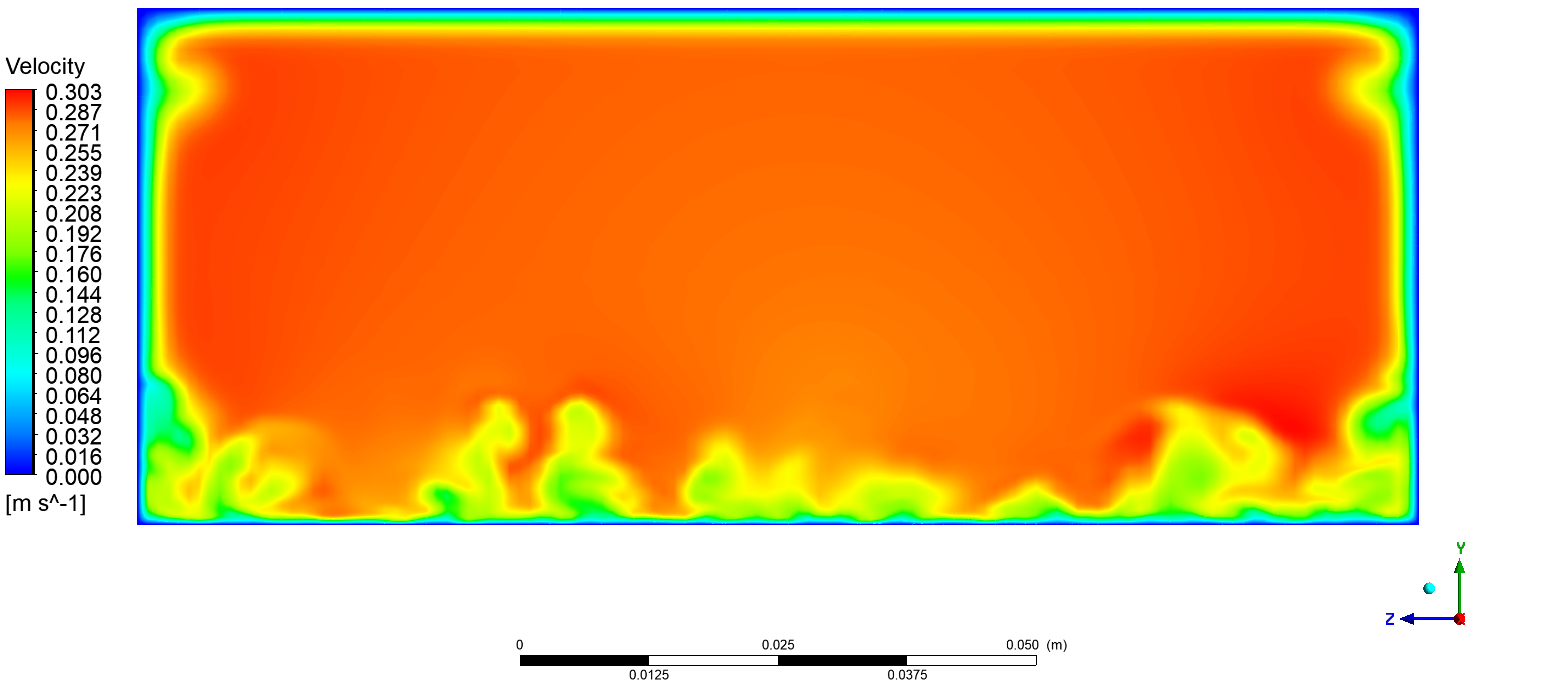
\includegraphics[width=1.1\linewidth]{../Assets/T665_Velocity_ContourYZ400}
		\caption{PlaneYZ400}
		\label{fig:T665VelocityContourYZ400}
	\end{subfigure}
	\\
	\begin{subfigure}{.5\textwidth}
		\centering
		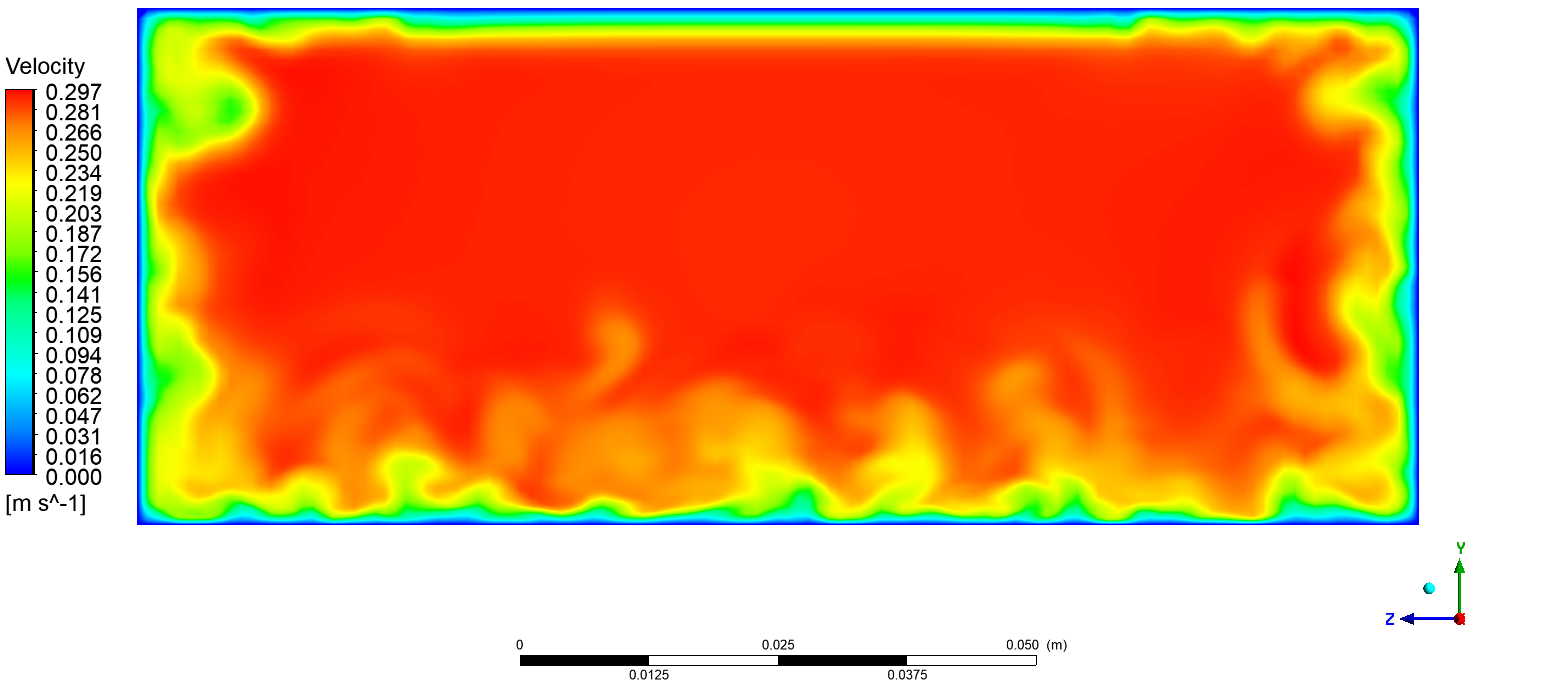
\includegraphics[width=1.1\linewidth]{../Assets/T665_Velocity_ContourYZ600}
		\caption{PlaneYZ600}
		\label{fig:T665VelocityContourYZ600}
	\end{subfigure}%
	\begin{subfigure}{.5\textwidth}
		\centering
		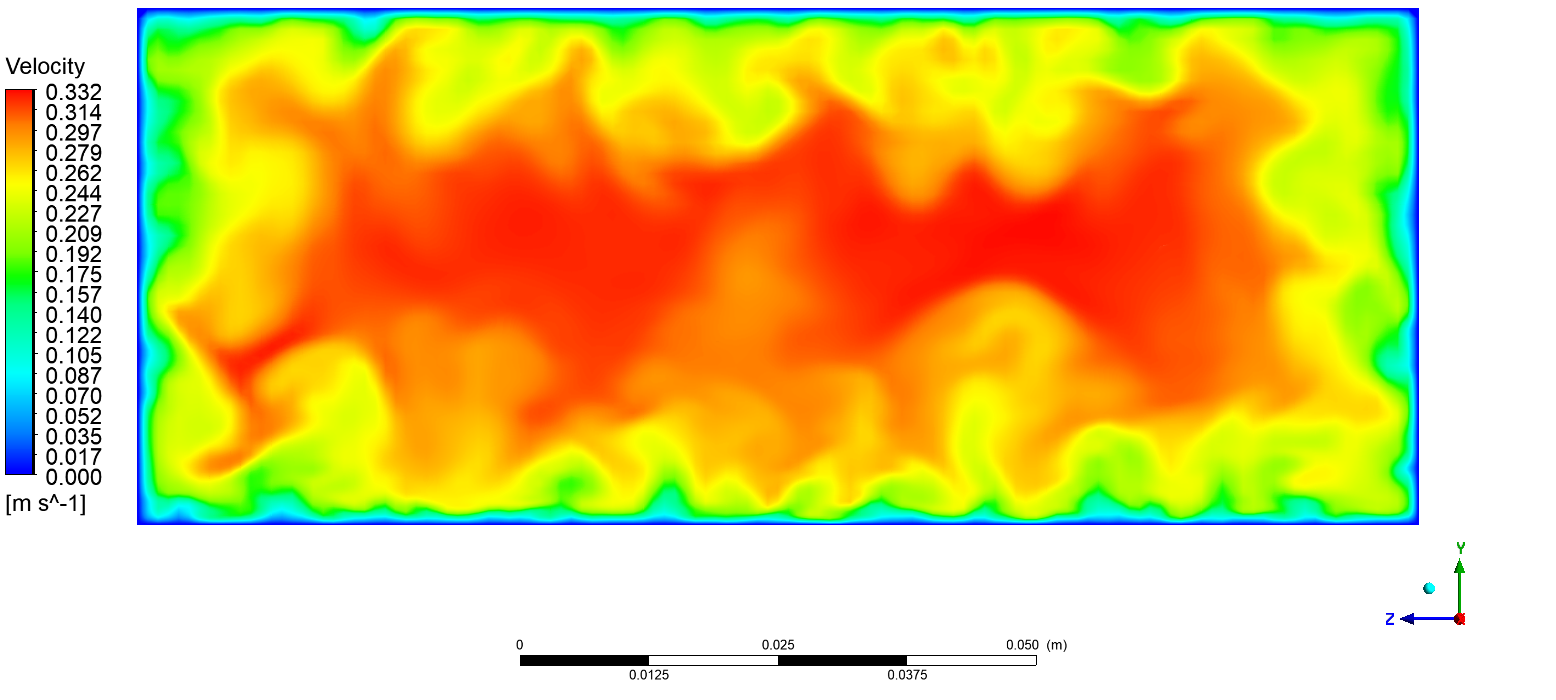
\includegraphics[width=1.1\linewidth]{../Assets/T665_Velocity_ContourYZ1400}
		\caption{PlaneYZ1400}
		\label{fig:T665VelocityContourYZ1400}
	\end{subfigure}
	\caption{Скорость в поперечных сечениях при t = 6.65 с}
	\label{fig:T665VelocityContourYZ}
\end{figure}
\begin{figure}[H]
	\centering
	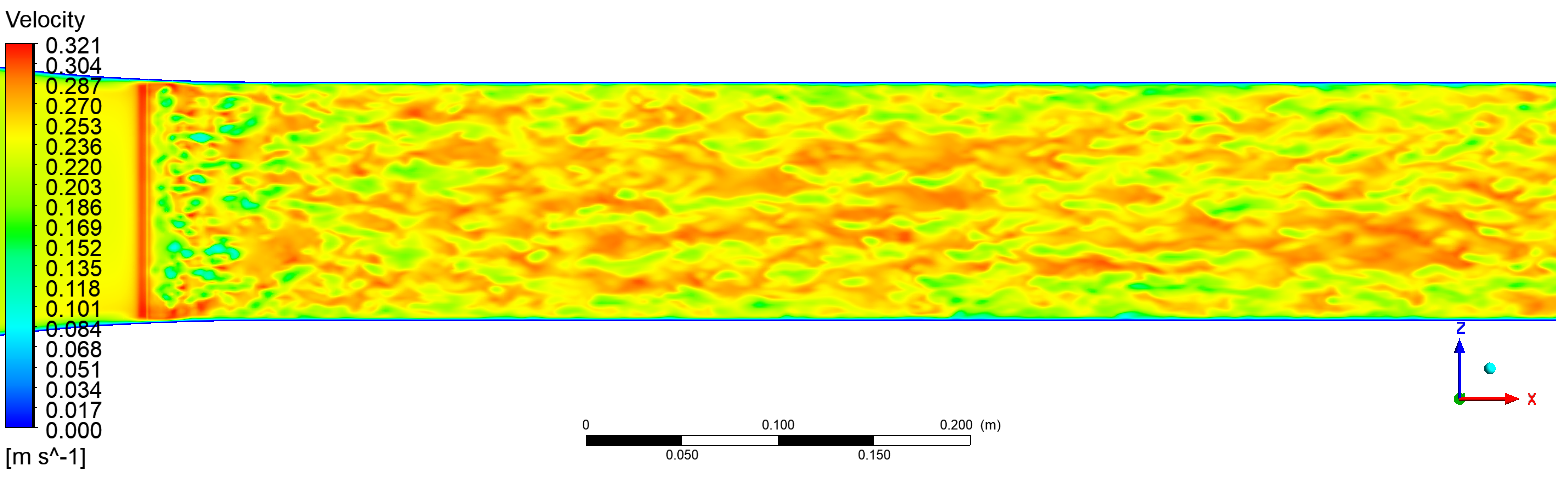
\includegraphics[width=1\linewidth]{../Assets/T665_Velocity_ContourXZ20M}
	\caption{PlaneXZ20M, t = 6.65 с}
	\label{fig:t665velocitycontourxz20m}
\end{figure}